

%----------
% DOCUMENT CONFIGURATION
%----------

\documentclass[12pt]{report} %font 12pt

% MARGINS
\usepackage[
a4paper,
vmargin=2.5cm,
hmargin=3cm
]{geometry}

\renewcommand{\baselinestretch}{1.15}
\parskip=6pt

% COLORS for cover and code
\usepackage[table]{xcolor}
\definecolor{azulUC3M}{RGB}{0,0,102}
\definecolor{gray97}{gray}{.97}
\definecolor{gray75}{gray}{.75}
\definecolor{gray45}{gray}{.45}

% Soporte para GENERAR PDF/A --es importante de cara a su inclusión en e-Archivo porque es el formato óptimo de preservación y a la generación de metadatos, tal y como se describe en http://uc3m.libguides.com/ld.php?content_id=31389625. En la carpeta incluímos el archivo plantilla_tfg_2017.xmpdata en el que puedes incluir los metadatos que se incorporarán al archivo PDF cuando lo compiles. Ese archivo debe llamarse igual que tu archivo .tex. Puedes ver un ejemplo en esta misma carpeta.
\usepackage[a-1b]{pdfx}

% LINKS
\usepackage{hyperref}
\hypersetup{colorlinks=true,
	linkcolor=black,
	urlcolor=blue}

% MATH
\usepackage{amsmath,amssymb,amsfonts,amsthm}

\usepackage{txfonts} 
\usepackage[T1]{fontenc}
\usepackage[utf8]{inputenc}

\usepackage[english]{babel} 
\usepackage[babel, english=american]{csquotes}
\AtBeginEnvironment{quote}{\small}

% FOOTER
\usepackage{fancyhdr}
\pagestyle{fancy}
\fancyhf{}
\renewcommand{\headrulewidth}{0pt}
\rfoot{\thepage}
\fancypagestyle{plain}{\pagestyle{fancy}}

% TITLES
\usepackage{titlesec}
\usepackage{titletoc}
\titleformat{\chapter}[block]
{\large\bfseries\filcenter}
{\thechapter.}
{5pt}
{\MakeUppercase}
{}
\titlespacing{\chapter}{0pt}{0pt}{*3}
\titlecontents{chapter}
[0pt]                                               
{}
{\contentsmargin{0pt}\thecontentslabel.\enspace\uppercase}
{\contentsmargin{0pt}\uppercase}                        
{\titlerule*[.7pc]{.}\contentspage}                 

\titleformat{\section}
{\bfseries}
{\thesection.}
{5pt}
{}
\titlecontents{section}
[5pt]                                               
{}
{\contentsmargin{0pt}\thecontentslabel.\enspace}
{\contentsmargin{0pt}}
{\titlerule*[.7pc]{.}\contentspage}

\titleformat{\subsection}
{\normalsize\bfseries}
{\thesubsection.}
{5pt}
{}
\titlecontents{subsection}
[10pt]                                               
{}
{\contentsmargin{0pt}                          
	\thecontentslabel.\enspace}
{\contentsmargin{0pt}}                        
{\titlerule*[.7pc]{.}\contentspage}  


% TABLE DESIGN
\usepackage{multirow}
\usepackage{caption}
\usepackage{floatrow} 
\usepackage{array}
\newcolumntype{P}[1]{>{\centering\arraybackslash}p{#1}}
\DeclareCaptionFormat{upper}{#1#2\uppercase{#3}\par}

\captionsetup[table]{
	%format=upper,  UPPER??? Set by the template, but it looks really weird, I got this off
	justification=centering,
	labelsep=period,
	width=.75\linewidth,
	labelfont=small,
	font=small,
}



% FIGURES DESIGN
\usepackage{graphicx}
\graphicspath{{images/}}

\captionsetup[figure]{
	format=hang,
	name=Fig.,
	singlelinecheck=off,
	labelsep=period,
	labelfont=small,
	font=small,
	%THE FOLLOWING WAS ADDED BY ME, is this ok? I think it was missed on the template
	justification=centering		
}


% FOOT NOTES
\usepackage{chngcntr}
\counterwithout{footnote}{chapter}

% CODE LISTINGS
\usepackage{listings}

\lstdefinestyle{estilo}{ frame=Ltb,
	framerule=0pt,
	aboveskip=0.5cm,
	framextopmargin=3pt,
	framexbottommargin=3pt,
	framexleftmargin=0.4cm,
	framesep=0pt,
	rulesep=.4pt,
	backgroundcolor=\color{gray97},
	rulesepcolor=\color{black},
	%
	basicstyle=\ttfamily\footnotesize,
	keywordstyle=\bfseries,
	stringstyle=\ttfamily,
	showstringspaces = false,
	commentstyle=\color{gray45},     
	%
	numbers=left,
	numbersep=15pt,
	numberstyle=\tiny,
	numberfirstline = false,
	breaklines=true,
	xleftmargin=\parindent
}

\captionsetup[lstlisting]{font=small, labelsep=period}

\lstset{style=estilo}
\renewcommand{\lstlistingname}{\uppercase{Code}}

% IEEE BIBLIOGRAPHY
\usepackage[backend=biber, style=ieee, isbn=false,sortcites, maxbibnames=5, minbibnames=1]{biblatex}

\addbibresource{bibliography/bibliography.bib}


%-------------
%	DOCUMENT
%-------------

\begin{document}
\pagenumbering{roman}
	
%----------
%	COVER
%----------	
\begin{titlepage}
	\begin{sffamily}
	\color{azulUC3M}
	\begin{center}
		\begin{figure}[H] %university logotype
			\makebox[\textwidth][c]{
\includegraphics[width=16cm]{Portada_Logo.png}}
		\end{figure}
		\vspace{2.5cm}
		\begin{Large}
			University Degree in Computer Science and Engineering\\			
			Academic Year 2021-2022\\
			\vspace{2cm}		
			\textsl{Bachelor Thesis}
			\bigskip
			
		\end{Large}
		 	{\Huge ``An analysis of offensive capabilities of eBPF and implementation of a rootkit''}\\
		 	\vspace*{0.5cm}
	 		\rule{10.5cm}{0.1mm}\\
			\vspace*{0.9cm}
			{\LARGE Marcos Sánchez Bajo}\\ 
			\vspace*{1cm}
		\begin{Large}
			Juan Manuel Estévez Tapiador\\
			Leganés, 2022\\
		\end{Large}
	\end{center}
	\vfill
	\color{black}
	% Creative Commons license
	
\includegraphics[width=4.2cm]{images/creativecommons.png}\\  
	This work is licensed under Creative Commons \textbf{Attribution – Non Commercial – Non Derivatives}
	\end{sffamily}
\end{titlepage}

\newpage
\thispagestyle{empty}
\mbox{}

%----------
%	SUMMARY & KEYWORDS
%----------	
\renewcommand\abstractname{\large\uppercase{Summary}}
\begin{abstract}
\thispagestyle{plain}
\setcounter{page}{3}
	
	% TODO SUMMARY
	
	\textbf{Keywords:}
	% TODO KEYWORDS
	
	\vfill
\end{abstract}
	\newpage
	\thispagestyle{empty}
	\mbox{}


%----------
%	DEDICATION
%----------	
\chapter*{Dedication}

\setcounter{page}{5}
	
	% TODO DEDICATION	
		
	\vfill
	
	\newpage
	\thispagestyle{empty}
	\mbox{}
	
\chapter*{Abstract}

\setcounter{page}{5}
	
	% TODO ABSTRACT	
		
	\vfill
	
	\newpage
	\thispagestyle{empty}
	\mbox{}
	

%----------
%	INDEXES
%----------	

%--
%General indexes
%-
\tableofcontents
\thispagestyle{fancy}

\newpage
\thispagestyle{empty}
\mbox{}

%--
% List of figures
%-
\listoffigures
\thispagestyle{fancy}

\newpage
\thispagestyle{empty}
\mbox{}

%--
% List of tables
%-
\listoftables
\thispagestyle{fancy}

\newpage % página en blanco o de cortesía
\thispagestyle{empty}
\mbox{}


%----------
%	INTRODUCTION
%----------	
\clearpage
\pagenumbering{arabic}

\chapter{Introduction}
\section{Motivation}
%M-> SA bit long, but it summarizes and presents the ideas and background needed to understand the topic in order:
% Main idea: Malware keeps evolving -> 
% -> Relevance of innovating and researching on the new techniques ->
% -> Relevance of stealth software in targeted attacks-> 
% -> Introduce eBPF as the logical step of innovation in the field ->
% -> There is a need to research on this topic now.

As the efforts of the computer security community grow to protect increasingly critical devices and networks from malware infections, so do the techniques used by malicious actors become more sophisticated. Following the incorporation of ever more capable firewalls and Intrusion Detection Systems (IDS), cybercriminals have in turn sought novel attack vectors and exploits in common software, taking advantage of an inevitably larger attack surface that keeps growing due to the continued incorporation of new programs and functionalities into modern computer systems.

In contrast with ransomware incidents, which remained the most significant and common cyber threat faced by organizations on 2021\cite{ransomware_pwc}, a powerful class of malware called rootkits is found considerably more infrequently, yet it is usually associated to high-profile targeted attacks that lead to greatly impactful consequences. 

A rootkit is a piece of computer software characterized for its advanced stealth capabilities. Once it is installed on a system it remains invisible to the host, usually hiding its related processes and files from the user, while at the same time performing the malicious operations for which it was designed. Common operations include storing keystrokes, sniffing network traffic, exfiltrating sensitive information from the user or the system, or actively modifying critical data at the infected device. The other characteristic functionality is that rootkits seek to achieve persistence on the infected hosts, meaning that they keep running on the system even after a system reboot, without further user interaction or the need of a new compromise.
The techniques used for achieving both of these functionalities depend on the type of rootkit developed, a classification usually made depending on the level of privileges on which the rootkit operates in the system.

\begin{itemize}
\item \textbf{User-mode} rootkits run at the same level of privilege as common user applications. They usually work by hijacking legitimate processes on which they may inject code by preloading shared libraries, thus modifying the calls issued to user APIs, on which malicious code is placed by the rootkit. Although easier to build, these rootkits are exposed to detection by common anti-malware programs.
%I am mentioning the kernel panic part because that could be considered an advantage for eBPF, there is less worry about crashing the system
\item \textbf{Kernel-mode} rootkits run at the same level of privilege as the operating system, thus enjoying unrestricted access to the whole computer. These rootkits usually come as kernel modules or device drivers and, once loaded, they reside in the kernel. This implies that special attention must be taken to avoid programming errors since they could potentially corrupt user or kernel memory, resulting in a fatal kernel panic and a subsequent system reboot, which goes against the original purpose of maintaining stealth.

Common techniques used for the development of their malicious activities include hooking system calls made to the kernel by user applications (on which malicious code is then injected), or modifying data structures in the kernel to change the data of user programs at runtime. Therefore, trusted programs on an infected machine can no longer be trusted to operate securely.

These rootkits are usually the most attractive (and difficult to build) option for a malicious actor, but the installation of a kernel rootkit requires of a complete previous compromise of the system, meaning that administrator or root privileges must have been already achieved by the attacker, commonly by the execution of an exploit or a local installation of a privileged user.
\end{itemize}

Historically, kernel-mode rootkits have been tightly associated with espionage activities on governments and research institutes by Advanced Persistent Threat (APT) groups\cite{rootkit_ptsecurity}, state-sponsored or criminal organizations specialized on long-term operations to gather intelligence and gain unauthorized persistent access to computer systems. Although rootkits' functionality is tailored for each specific attack, a common set of techniques and procedures can be identified being used by these organizations. However, during the last years, a new technology called eBPF has been found to be the heart of the latest innovation on the development of rootkits. 

%Yes, I am not mentioning that eBPF comes from "Extended Berkeley Packet %Filters here since apparently it is no longer considered an acronym, we'll %tackle that on the history section
eBPF is a technology incorporated in the 3.18 version of the Linux kernel\cite{ebpf_linux318}, which provides the possibility of running code in the kernel without the need of loading a kernel module. Programs are created in a restrictive version of the C language and compiled into eBPF bytecode, which is loaded into the kernel via a new bpf() system call. After a mandatory step of verification by the kernel in which the code is checked to be safe to run, the bytecode is compiled into native machine instructions. These programs can then get access to kernel-exclusive functionalities including network traffic filtering, system calls hooking or tracing.

Although eBPF has built an outstanding environment for the creation of networking and tracing tools, its ability to run kernel programs without the need to load a kernel module has attracted the attention of multiple APTs. On February 2022, the Chinese security team Pangu Lab reported about a NSA backdoor that remained unnoticed since 2013 that used eBPF for its networking functionality and that infected military and telecommunications systems worldwide\cite{bvp47_report}. Also on 2022, PwC reports about a China-based threat actor that has targeted telecommunications systems with a eBPF-based backdoor\cite{bpfdoor_pwc}.

Moreover, there currently exists official efforts to extend the eBPF technology into Windows\cite{ebpf_windows} and Android systems\cite{ebpf_android}, which spreads the mentioned risks to new platforms. Therefore, we can confidently claim that there is a growing interest on researching the capabilities of eBPF in the context of offensive security, in particular given its potential on becoming a common component found of modern rootkits. This knowledge would be valuable to the computer security community, both in the context of pen-testing and for analysts which need to know about the latest trends in malware to prepare their defences.


\section{Project objectives}
The main objective of this project is to compile a comprehensive report of the capabilities in the eBPF technology that could be weaponized by a malicious actor. In particular, we will be focusing on functionalities present in the Linux platform, given the maturity of eBPF on these environments and which therefore offers a wider range of possibilities. We will be approaching this study from the perspective of a threat actor, meaning that we will develop an eBPF-based rootkit which shows these capabilities live in a current Linux system, including proof of concepts (PoC) showing an specific feature, and also by building a realistic rootkit system which weaponizes these PoCs and operates malicious activities. 

%According to the library guide, previous research should be around here. %Is it the best place tho?
Before narrowing down our objectives and selecting an specific list of rootkit capabilities to emulate using eBPF, we needed to consider previous research. The work on this matter by Jeff Dileo from NCC Group at DEFCON 27\cite{evil_ebpf} is particularly relevant, setting the first basis of eBPF ability to overwrite userland data, highlighting the possibility of overwriting the memory of a running process and executing arbitrary code on it.

Subsequent talks on 2021 by Pat Hogan at DEFCON 29\cite{bad_ebpf}, and by Guillaume Fournier and Sylvain Afchainthe from Datadog at DEFCON 29\cite{ebpf_friends}, research deeper on eBPF's ability to behave like a rootkit. In particular, Hogan shows how eBPF can be used to hide the rootkit's presence from the user and to modify data at system calls, whilst Fournier and Afchainthe built the first instance of an eBPF-based backdoor with command-and-control(C2) capabilities, enabling to communicate with the malicious eBPF program by sending network packets to the compromised machine.

Taking the previous research into account, and on the basis of common functionality we described to be usually incorporated at rootkits, the objectives of our research on eBPF is set to be on the following topics:
\begin{itemize}
\item Analysing eBPF's possibilities when hooking system calls and kernel functions.
\item Learning eBPF's potential to read/write arbitrary memory.
\item Exploring networking capabilities with eBPF packet filters.
\end{itemize}

The knowledge gathered by the previous three pillars will be then used as a basis for building our rootkit. We will present attack vectors and techniques different than the ones presented in previous research, although inevitably we will also tackle common points, which will be clearly indicated and on which we will try to perform further research. In essence, our eBPF-based rootkit aims at:
\begin{itemize}
\item Hijacking the execution of user programs while they are running, injecting libraries and executing malicious code, without impacting their normal execution.
\item Featuring a command-and-control module powered by a network backdoor, which can be operated from a remote client. This backdoor should be controlled with stealth in mind, featuring similar mechanisms to those present in rootkits found in the wild.
\item Tampering with user data at system calls, resulting in running malware-like programs and for other malicious purposes.
\item Achieving stealth, hiding rootkit-related files from the user.
\item Achieving rootkit persistence, the rootkit should run after a complete system reboot.
\
\end{itemize}

The rootkit will work in a fresh-install of a Linux system with the following characteristics:
\begin{itemize}
%Maybe a table for this?
\item Distribution: Ubuntu 21.04.
\item Kernel version: 5.11.0-49.
\end{itemize} 

\section{Regulatory framework}
%MARCOS-> Is this the appropiate place? Looking at other TFGs it is sometimes here and others in a final chapter

%TODO - Leaving this for the end

\subsection{Social and economic environment}
%M-> Mentioned talking about community outreach and its role under pentesting

%TODO - Leaving this for the end

\subsection{Budget}
%TODO - Leaving this for the end

\section{Structure of the document}
%TODO - Best to be done at the end


%%%%%%%%%%%%%%%
%TODO IMPORTANT- Clearly structure eveything, for instance I am not sure about the "Methods" section. Maybe a "State of the Art"+"Analysis of offensive capabilities"+"Implementation of a rootkit" is more suitable?
%I'm following that for now, we can join it together afterwards if it was not a good idea.
%
% In the end, we need to talk about 3 main points before the conclusion at least:
% 1- Background on eBPF, what it is, how it works. How we will develop applications on it(libbpf).
% 2- Offensive capabilities of ebpf
% 3- Our rootkit in ebpf with the previous section as the basis. The idea is to show diagrams with the components and describe the functionality. However, the library injection part is long and requires quite a background by itself. Should we introduce the background on a different section??
%%%%%%%%%%%%%%

\chapter{State of the art}
% I WILL NOT INCLUDE A ROOTKIT BACKGROUND, considering that a deep study of that is not fully relevant for us. I explained what it is, its two main types (should we include bootkits, maybe?) and its relation with eBPF in the introduction, since it is needed to introduce the overall context. Should we do otherwise?
This chapter is dedicated to an study of the eBPF technology. Firstly, we will analyse its origins, understanding what it is and how it works, and discuss the reasons why it is a necessary component of the Linux kernel today. Afterwards, we will cover the main features of eBPF in detail. Finally, an study of the existing alternatives for developing eBPF applications will be also included.

Although during our discussion of the offensive capabilities of eBPF in section\ref{section:analysis_offensive_capabilities} we will use a library that will provide us with a layer of abstraction over the underlying operations, this background is needed to understand how eBPF is embedded in the kernel and which capabilities and limits we can expect to achieve with it.

\section{eBPF history - Classic BPF}
% Is it ok to have sections / chapters without individual intros?
In this section we will detail the origins of eBPF in the Linux kernel. By offering us background into the earlier versions of the system, the goal is to acquire insight on the design decisions included in modern versions of eBPF.

\subsection{Introduction to the BPF system}
Nowadays eBPF is not officially considered to be an acronym anymore\cite{ebpf_io}, but it remains largely known as "extended Berkeley Packet Filters", given its roots in the Berkeley Packet Filter (BPF) technology, now known as classic BPF.

BPF was introduced in 1992 by Steven McCanne and Van Jacobson in the paper "The BSD Packet Filter: A New Architecture for User-level Packet Capture"\cite{bpf_bsd_origin}, as a new filtering technology for network packets in the BSD platform. It was first integrated in the Linux kernel on version 2.1.75\cite{ebpf_history_opensource}.


\begin{figure}[H]
	\centering
	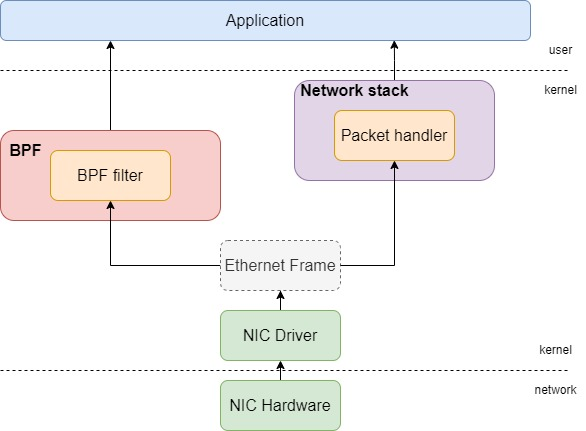
\includegraphics[width=12cm, keepaspectratio=true]{classic_bpf.jpg}
	\caption{Sketch of the functionality of classic BPF}
	\label{fig:classif_bpf}
\end{figure}

Figure \ref{fig:classif_bpf} shows how BPF was integrated in the existing network packet processing by the kernel. After receiving a packet via the Network Interface Controller (NIC) driver, it would first be analysed by BPF filters, which are programs directly developed by the user. This filter decides whether the packet is to be accepted by analysing the packet properties, such as its length or the type and values of its headers. If a packet is accepted, the filter proceeds to decide how many bytes of the original buffer are passed to the application at the user space. Otherwise, the packet is redirected to the original network stack, where it is managed as usual.


\subsection{The BPF virtual machine} \label{subsection:bpf_vm}
In a technical level, BPF comprises both the BPF filter programs developed by the user and the BPF module included in the kernel which allows for loading and running the BPF filters. This BPF module in the kernel works as a virtual machine\cite{bpf_bsd_origin_bpf_page1}, meaning that it parses and interprets the filter program by providing simulated components needed for its execution, turning into a software-based CPU. Because of this reason, it is usually referred as the BPF Virtual Machine (BPF VM). The BPF VM comprises the following components:
\begin{itemize}
\item \textbf{An accumulator register}, used to store intermediate values of operations.
\item \textbf{An index register}, used to modify operand addresses, it is usually incorporated to optimize vector operations\cite{index_register}.
\item \textbf{An scratch memory store}, a temporary storage.
\item \textbf{A program counter}, used to point to the next machine instruction to execute in a filter program.
\end{itemize}


\subsection{Analysis of a BPF filter program} \label{subsection:analysis_bpf_filter_prog}
As we mentioned in section \ref{subsection:bpf_vm}, the components of the BPF VM are used to support running BPF filter programs. A BPF filter is implemented as a boolean function:
\begin{itemize}
\item If it returns \textit{true}, the kernel copies the packet to the application.
\item If it returns \textit{false}, the packet is not accepted by the filter (and thus the network stack will be the next to operate it).
\end{itemize}

\begin{figure}[H]
	\centering
	\includegraphics[width=8cm]{cbpf_prog.jpg}
	\caption{Execution of a BPF filter.}
	\label{fig:cbpf_prog}
\end{figure}

Figure \ref{fig:cbpf_prog} shows an example of a BPF filter upon receiving a packet. In the figure, green lines indicate that the condition is true and red lines that it is evaluated as false. Therefore, the execution works as a control flow graph (CFG) which ends on a boolean value\cite{bpf_bsd_origin_bpf_page5}. The figure presents an example BPF program which accepts the following frames:
\begin{itemize}
\item Frames with an IP packet as a payload directed from IP address X.
\item Frames with an IP packet as a payload directed towards IP address Y.
\item Frames belonging to the ARP protocol and from IP address Y.
\item Frames not from the ARP protocol directed from IP address Y to IP address X.
\end{itemize}


\subsection{BPF bytecode instruction format}
In order to implement the CFG to be run at the BPF VM, BPF filter programs are made up of BPF bytecode, which is defined by a new BPF instruction set. Therefore, a BPF filter program is an array of BPF bytecode instructions\cite{bpf_organicprogrammer_analysis}.


\begin{table}[H]
\begin{tabular}{|c|c|c|c|c|}
\hline
& OPCODE & JT & JF & K\\
\hline
BITS & 16 & 8 & 8 & 32\\
\hline
\end{tabular}
\caption{Table showing BPF instruction format. It is a fixed-length 64 bit instruction, the number of bits used by each field are indicated.}
\label{table:bpf_inst_format}
\end{table}

Table \ref{table:bpf_inst_format} shows the format of a BPF bytecode instruction. As it can be observed, it is a compound of:
\begin{itemize}
\item An \textbf{opcode}, similar to assembly opcode, it indicates the operation to be executed.
\item Field \textbf{jt} indicates the offset to the next instruction to jump in case a condition is evaluated as \textit{true}.
\item Field \textbf{jf} indicates the offset to the next instruction to jump in case a condition is evaluated as \textit{false}.
\item Field \textbf{k} is miscellaneous and its contents vary depending on the instruction opcode.
\end{itemize}

\begin{figure}[H]
	\centering
	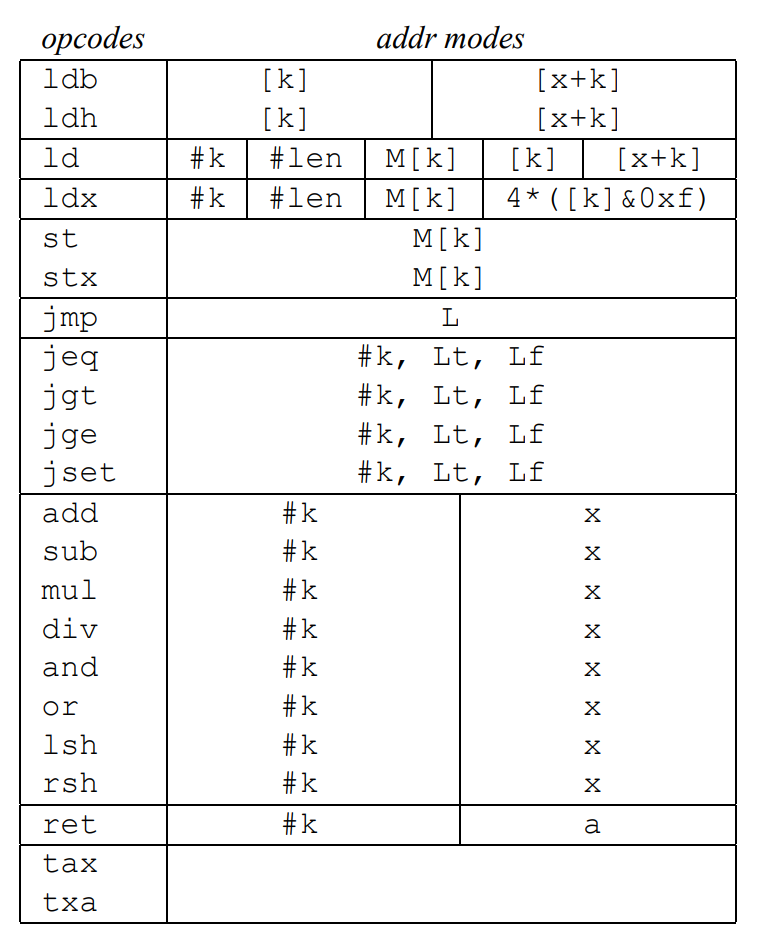
\includegraphics[width=8cm]{bpf_instructions.png}
	\caption{Table of supported classic BPF instructions, as shown by McCanne and Jacobson\cite{bpf_bsd_origin_bpf_page7}}
	\label{fig:bpf_instructions}
\end{figure}

Figure \ref{fig:bpf_instructions} shows how BPF instructions are defined according to the BPF instruction set. As we mentioned, similarly to assembly, instructions include an opcode which indicates the operation to execute, and the multiple arguments defining the arguments of the operation. The table shows, in order by rows, the following instruction types\cite{bpf_bsd_origin_bpf_page8}:
\begin{itemize}
\item Rows 1-4 are \textbf{load instructions}, copying the addressed value into the index or accumulator register.
\item Rows 4-6 are \textbf{store instructions}, copying the accumulator or index register into the scratch memory store.
\item Rows 7-11 are \textbf{jump instructions}, changing the program counter register. These are usually present on each node of the CFG, and evaluate whether the condition to be evaluated is true or not.
\item Rows 12-19 and 21-22 are \textbf{arithmetic and miscellaneous instructions}, performing operations usually needed during the program execution.
\item Row 20 is a \textbf{return instruction}, it is positioned in the final end of the CFG, and indicate whether the filter accepts the packet (returning true) or otherwise rejects it (return false).
\end{itemize}

\begin{figure}[H]
	\centering
	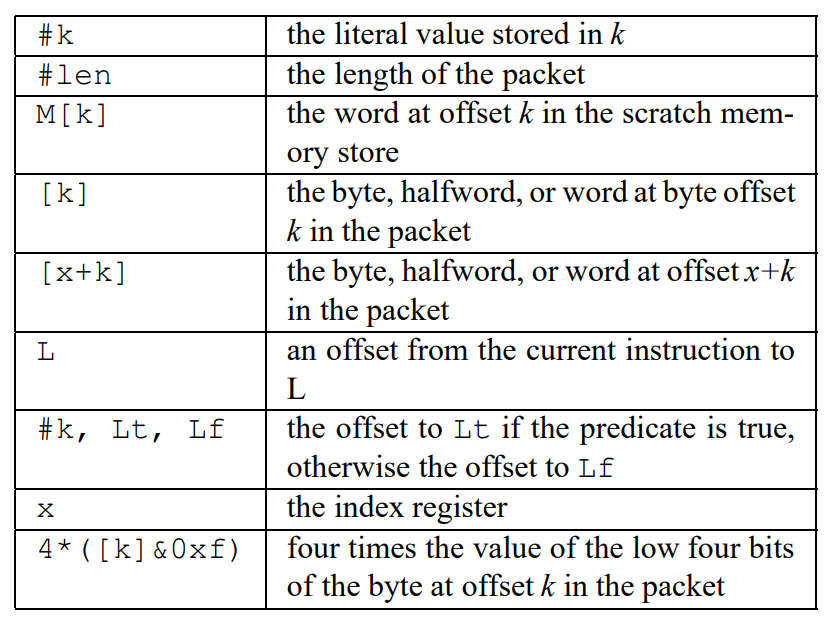
\includegraphics[width=8cm]{bpf_address_mode.png}
	\caption{Table explaining the column address modes in Figure\ref{fig:bpf_instructions}, as shown by McCanne and Jacobson\cite{bpf_bsd_origin_bpf_page8}}
	\label{fig:bpf_address_mode}
\end{figure}

The column \textit{addr modes} in figure \ref{fig:bpf_instructions} describes how the parameters of a BPF instruction are referenced depending on the opcode. The address modes are detailed in figure \ref{fig:bpf_address_mode}. As it can be observed, paremeters may consist of immediate values, offsets to memory positions or on the packet, the index register or combinations of the previous.


\subsection{An example of BPF filter with tcpdump}
At the time, by filtering packets before they are handled by the kernel instead of using an user-level application, BPF offered a performance improvement between 10 and 150 times the state-of-the art technologies of the moment\cite{bpf_bsd_origin_bpf_page1}. Since then, multiple popular tools began to use BPF, such as the network tracing tool \textit{tcpdump}\cite{tcpdump_page}.

\textit{tcpdump} is a command-line tool that enables to capture and analyse the network traffic going through the system. It works by setting filters on a network interface, so that it shows the packets that are accepted by the filter. Still today, \textit{tcpdump} uses BPF for the filter implementation. We will now show an example of BPF code used by \textit{tcpdump} to implement a simple filter:

\begin{figure}[H]
	\centering
	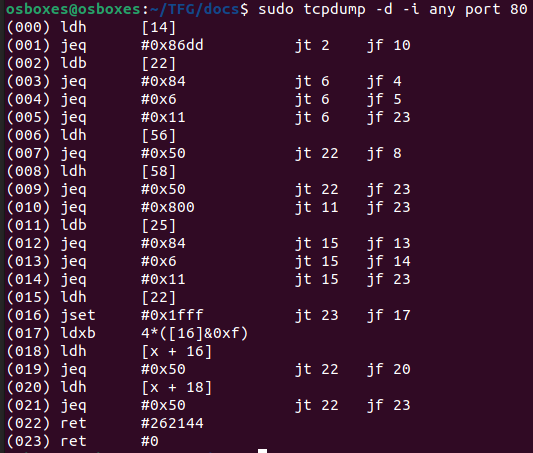
\includegraphics[width=10cm]{tcpdump_example.png}
	\caption{BPF bytecode tcpdump needs to set a filter to display packets directed to port 80.}
	\label{fig:bpf_tcpdump_example}
\end{figure}

Figure \ref{fig:bpf_tcpdump_example} shows how tcpdump sets a filter to display traffic directed to all interfaces (\textit{-i any}) directed to port 80. Flag \textit{-d} instructs tcpdump to display BPF bytecode.

In the example, using the \textit{jf} and \textit{jt} fields, we can label the nodes of the CFG described by the BPF filter. Figure \ref{fig:tcpdump_ex_sol} describes the shortest graph path that a true comparison will need to follow to be accepted by the filter. Note how instruction 010 is checking the value 80, the one our filter is looking for in the port.

\begin{figure}[H]
	\centering
	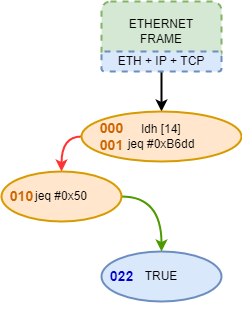
\includegraphics[width=6cm]{cBPF_prog_ex_sol.png}
	\caption{Shortest path in the CFG described in the example of figure \ref{fig:bpf_tcpdump_example} that a packet needs to follow to be accepted by the BPF filter set with \textit{tcpdump}.}
	\label{fig:tcpdump_ex_sol}
\end{figure}

\section{Analysis of modern eBPF} \label{section:modern_ebpf}
This section discusses the current state of modern eBPF in the Linux kernel. By building on the previous architecture described in classic BPF, we will be able to provide a comprehensive picture of the underlying infrastructure in which eBPF relies today.

The addition of classic BPF in the Linux kernel set the foundations of eBPF, but nowadays it has already extended its presence to many other components other than traffic filtering. Similarly to how BPF filters were included in the networking module of the Linux kernel, we will now study the necessary changes made in the kernel to support these new program types. Table \ref{table:ebpf_history} shows the main updates that were incorporated and shaped modern eBPF of today.

\begin{table}[H]
\begin{tabular}{|c|c|c|}
\hline
Description & Kernel version & Year\\
\hline
\hline
\textit{BPF}: First addition in the kernel & 2.1.75 & 1997\\
\textit{BPF+}: New JIT assembler & 3.0 & 2011\\
\textit{eBPF}: Added eBPF support & 3.15 & 2014\\
\textit New bpf() syscall & 3.18 & 2014\\
\textit Introduction of eBPF maps & 3.19 & 2015\\
\textit eBPF attached to kprobes & 4.1 & 2015\\
\textit Introduction of Traffic Control & 4.5 & 2016\\
\textit eBPF attached to tracepoints & 4.7 & 2016\\
\textit Introduction of XDP & 4.8 & 2016\\


\hline
\end{tabular}
\caption{Table showing relevant eBPF updates. Note that only those relevant for our research objectives are shown. This is a selection of the official complete table at \cite{ebpf_funcs_by_ver}.}
\label{table:ebpf_history}
\end{table}

As it can be observed in the table above, the main breakthrough happened in the 3.15 version, where Alexei Starovoitov, along with Daniel Borkmann, decided to expand the capabilities of BPF by remodelling the BPF instruction set and overall architecture\cite{brendan_gregg_bpf_book}.

Figure \ref{fig:ebpf_architecture} offers an overview of the current eBPF architecture. During the subsequent subsections, we will proceed to explain its components in detail.

\begin{figure}[H]
	\centering
	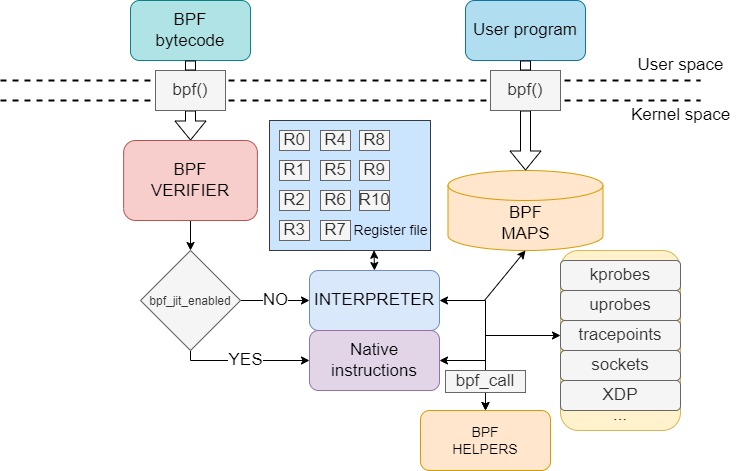
\includegraphics[width=15cm]{ebpf_arch.jpg}
	\caption{Figure showing overall eBPF architecture in the Linux kernel and the process of loading an eBPF program. Based on\cite{brendan_gregg_bpf_book} and \cite{ebpf_io_arch}.}
	\label{fig:ebpf_architecture}
\end{figure}

\subsection{eBPF instruction set} \label{subsection:ebpf_inst_set}
The eBPF update included a complete remodel of the instruction set architecture (ISA) of the BPF VM. Therefore, eBPF programs will need to follow the new architecture in order to be interpreted as valid and executed.

\begin{table}[H]
\begin{tabular}{|c|c|c|c|c|c|}
\hline
& IMM & OFF & SRC & DST & OPCODE \\
\hline
BITS & 32 & 16 & 4 & 4 & 8\\
\hline
\end{tabular}
\caption{Table showing eBPF instruction format. It is a fixed-length 64 bit instruction, the number of bits used by each field are indicated.}
\label{table:ebpf_inst_format}
\end{table}


Table \ref{table:ebpf_inst_format} shows the new instruction format for eBPF programs\cite{ebpf_inst_set}. The new fields are similar to x86\_64 assembly, incorporating the typically found immediate and offset fields, and source and destination registers\cite{8664_inst_set_specs}. Similarly, the instruction set is extended to be similar to the one typically found on x86\_64 systems, the complete list can be consulted in the official documentation\cite{ebpf_inst_set}.
%Should I talk about assembly or this more in detail?

With respect to the BPF VM registers, they get extended from 32 to 64 bits of length, and the number of registers is incremented to 10, instead of the original accumulator and index registers. These registers are also adapted to be similar to those in assembly, as it is shown in table \ref{table:ebpf_regs}.

\begin{table}[H]
\begin{tabular}{|c|c|m{21em}|}
\hline
eBPF register & x86\_64 register & Purpose\\
\hline
r0 & rax & Return value from functions and exit value of eBPF programs\\
r1 & rdi & Function call argument 1\\
r2 & rsi & Function call argument 2\\
r3 & rdx & Function call argument 3\\
r4 & rcx & Function call argument 4\\
r5 & r8 & Function call argument 5\\
r6 & rbx & Callee saved register, value preserved between calls\\
r7 & r13 & Callee saved register, value preserved between calls\\
r8 & r14 & Callee saved register, value preserved between calls\\
r9 & r15 & Callee saved register, value preserved between calls\\
r10 & rbp & Frame pointer for stack, read only\\
\hline
\end{tabular}
\caption{Table showing eBPF registers and their purpose in the BPF VM.\cite{ebpf_inst_set}\cite{ebpf_starovo_slides}.}
\label{table:ebpf_regs}
\end{table}

\subsection{JIT compilation}
We mentioned in subsection \ref{subsection:ebpf_inst_set} that eBPF registers and instructions describe an almost one-to-one correspondence to those in x86 assembly. This is in fact not a coincidence, but rather it is with the purpose of improving a functionality that was included in Linux kernel 3.0, called Just-in-Time (JIT) compilation\cite{ebpf_JIT}\cite{ebpf_JIT_demystify_page13}.

JIT compiling is an extra step that optimizes the execution speed of eBPF programs. It consists of translating BPF bytecode into machine-specific instructions, so that they run as fast as native code in the kernel. Machine instructions are generated during runtime, written directly into executable memory and executed there\cite{ebpf_JIT_demystify_page14}.

Therefore, when using JIT compiling (a setting defined by the variable \textit{bpf\_jit\_enable}\cite{jit_enable_setting}, BPF registers are translated into machine-specific registers following their one-to-one mapping and bytecode instructions are translated into machine-specific instructions\cite{ebpf_starovo_slides_page23}. There no longer exists an interpretation step by the BPF VM, since we can execute the code directly\cite{brendan_gregg_bpf_book_bpf_vm}.

The programs developed during this project will always have JIT compiling active.


\subsection{The eBPF verifier}
We introduced in figure \ref{fig:ebpf_architecture} the presence of the so-called eBPF verifier. Provided that we will be loading programs in the kernel from user space, these programs need to be checked for safety before being valid to be executed.

The verifier performs a series of tests which every eBPF program must pass in order to be accepted. Otherwise, user programs could leak privileged data, result in kernel memory corruption, or hang the kernel in an infinite loop, between others. Therefore, the verifier limits multiple aspects of eBPF programs so that they are restricted to the intended functionality, whilst at the same time offering a reasonable amount of freedom to the developer.

The following are the most relevant checks that the verifier performs in eBPF programs\cite{ebpf_verifier_kerneldocs}\cite{ebpf_JIT_demystify_page17-22}:
\begin{itemize}
\item Tests for ensuring overall control flow safety:
	\subitem No loops allowed (bounded loops accepted since kernel version 5.3\cite{ebpf_bounded_loops}.
	\subitem Function call and jumps safety to known, reachable functions.
\item Tests for individual instructions:
	 \subitem Divisions by zero and invalid shift operations.
	 \subitem Invalid stack access and invalid out-of-bound access to data structures.
	 \subitem Reads from uninitialized registers and corruption of pointers.
\end{itemize}

These checks are performed by two main algorithms:
\begin{itemize}
\item Build a graph representing the eBPF instructions (similar to the one shown in section \ref{subsection:analysis_bpf_filter_prog}. Check that it is in fact a direct acyclic graph (DAG), meaning that the verifier prevents loops and unreachable instructions.
\item Simulate execution flow by starting on the first instruction and following each possible path, observing at each instruction the state of every register and of the stack.
\end{itemize}

\subsection{eBPF maps} \label{subsection:ebpf_maps}
An eBPF map is a generic storage for eBPF programs used to share data between user and kernel space, to maintain persistent data between eBPF calls and to share information between multiple eBPF programs\cite{ebpf_maps_kernel}.

A map consists of a key + value tuple. Both fields can have an arbitrary data type, the map only needs to know the length of the key and the value field at its creation\cite{bpf_syscall}. Programs can open maps by specifying their ID, and lookup or delete elements in the map by specifying its key, also insert new ones by supplying the element value and they key to store it with.

Therefore, creating a map requires a struct with the following fields:

\begin{table}[H]
\begin{tabular}{|c|c|}
\hline
FIELD & VALUE\\
\hline
type & Type of eBPF map. Described in table \ref{table:ebpf_map_types}\\
key\_size & Size of the data structure to use as a key\\
value\_size & Size of the data structure to use as value field\\
max\_entries & Maximum number of elements in the map\\
\hline
\end{tabular}
\caption{Table showing common fields for creating an eBPF map.}
\label{table:ebpf_map_struct}
\end{table}

\begin{table}[H]
\begin{tabular}{|c|>{\centering\arraybackslash}p{10cm}|}
\hline
TYPE & DESCRIPTION\\
\hline
BPF\_MAP\_TYPE\_HASH & A hast table-like storage, elements are stored in tuples.\\
BPF\_MAP\_TYPE\_ARRAY & Elements are stored in an array.\\
BPF\_MAP\_TYPE\_RINGBUF & Map providing alerts from kernel to user space, covered in subsection \ref{subsection:bpf_ring_buf}\\
BPF\_MAP\_TYPE\_PROG\_ARRAY & Stores descriptors of eBPF programs\\
\hline
\hline
\end{tabular}
\caption{Table showing types of eBPF maps. Only those used in our rootkit are displayed, the full list can be consulted in the man page \cite{bpf_syscall}}
\label{table:ebpf_map_types}
\end{table}

Table \ref{table:ebpf_maps} describes the main types of eBPF maps that are available for use. During the development of our rootkit, we will mainly focus on hash maps (BPF\_MAP\_TYPE\_HASH), provided that they are simple to use and we do not require of any special storage for our research purposes.

\subsection{The eBPF ring buffer} \label{subsection:bpf_ring_buf}
eBPF ring buffers are a special kind of eBPF maps, providing a one-way directional communication system, going from an eBPF program in the kernel to an user space program that subscribes to its events.

%TODO DIAGRAM OF A TYPICAL RING BUFFER

\subsection{The bpf() syscall} \label{subsection:bpf_syscall}
The bpf() syscall is used to issue commands from user space to kernel space in eBPF programs. This syscall is multiplexor, meaning that it can perform a great range of actions, changing its behaviour depending on the parameters.

The main operations that can be issued are described in table \ref{table:bpf_syscall}:

\begin{table}[H]
\begin{tabular}{|c|>{\centering\arraybackslash}p{5cm}|>{\centering\arraybackslash}p{5cm}|}
\hline
COMMAND & ATTRIBUTES & DESCRIPTION\\
\hline
\hline
BPF\_MAP\_CREATE & Struct with map info as defined in table \ref{table:ebpf_map_struct} & Create a new map\\
\hline
BPF\_MAP\_LOOKUP\_ELEM & Map ID, and struct with key to search in the map & Get the element on the map with an specific key\\
\hline
BPF\_MAP\_UPDATE\_ELEM & Map ID, and struct with key and new value & Update the element of an specific key with a new value\\
\hline
BPF\_MAP\_DELETE\_ELEM & Map ID and struct with key to search in the map & Delete the element on the map with an specific key\\
\hline
BPF\_PROG\_LOAD & Struct describing the type of eBPF program to load & Load an eBPF program in the kernel\\
\hline
\end{tabular}
\caption{Table showing types of syscall actions. Only those relevant to our research are shown the full list and attribute details can be consulted in the man page \cite{bpf_syscall}}
\label{table:ebpf_syscall}
\end{table}

With respect to the program type indicated with BPF\_PROG\_LOAD, this parameter indicates the type of eBPF program, setting the context in the kernel in which it will run, and to which modules it will have access to. The types of programs relevant for our research are described in table \ref{table:ebpf_prog_types}.

\begin{table}[H]
\begin{tabular}{|c|>{\centering\arraybackslash}p{5cm}|}
\hline
PROGRAM TYPE & DESCRIPTION\\
\hline
\hline
BPF\_PROG\_TYPE\_KPROBE & Program to instrument code to an attached kprobe\\
\hline
BPF\_PROG\_TYPE\_UPROBE & Program to instrument code to an attached uprobe\\
\hline
BPF\_PROG\_TYPE\_TRACEPOINT & Program to instrument code to a syscall tracepoint\\
\hline
BPF\_PROG\_TYPE\_XDP & Program to filter, redirect and monitor network events from the Xpress Data Path\\
\hline
BPF\_PROG\_TYPE\_SCHED\_CLS & Program to filter, redirect and monitor events using the Traffic Control classifier\\
\hline
\end{tabular}
\caption{Table showing types of eBPF programs. Only those relevant to our research are shown. The full list and attribute details can be consulted in the man page \cite{bpf_syscall}.}
\label{table:ebpf_prog_types}
\end{table}

In section \ref{section:TODO}, we will proceed to analyse in detail the different program types and what capabilities` they offer.

\subsection{eBPF helpers} \label{subsection:ebpf_helpers}
Our last component to cover of the eBPF architecture are the eBPF helpers. Since eBPF programs have limited accessibility to kernel functions (which kernel modules commonly have free access to), the eBPF system offers a set of limited functions called helpers\cite{ebpf_helpers}, which are used by eBPF programs to perform certain actions and interact with the context on which they are run. The list of helpers a program can call varies between eBPF program types, since different programs run in different contexts.

It is important to highlight that, just like commands issued via the bpf() syscall can only be issued from the user space, eBPF helpers correspond to the kernel-side of eBPF program exclusively. Note that we will also find a symmetric correspondence to those functions of the bpf() syscall related to map operations (since these are accessible both from user and kernel space).

Table \ref{table:ebpf_helpers} lists the most relevant general-purpose eBPF helpers we will use during the development of our project. We will later detail those helpers exclusive to an specific eBPF program type in the sections on which they are studied.

\begin{table}[H]
\begin{tabular}{|c|>{\centering\arraybackslash}p{10cm}|}
\hline
eBPF helper & DESCRIPTION\\
\hline
\hline
bpf\_map\_lookup\_elem() & Query an element with a certain key in a map\\
\hline
bpf\_map\_delete\_elem() & Delete an element with a certain key in a map\\
\hline
bpf\_map\_update\_elem() & Update the value of the element with a certain key in a map\\
\hline
bpf\_probe\_read\_user() & Attempt to safely read data at an specific user address into a buffer\\
\hline
bpf\_probe\_read\_kernel() & Attempt to safely read data at an specific kernel address into a buffer\\
\hline
bpf\_trace\_printk() & Similarly to printk() in kernel modules, writes buffer in \/sys\/kernel\/debug\/tracing\/trace\_pipe\\
\hline
bpf\_get\_current\_pid\_tgid() & Get the process process id (PID) and thread group id (TGID)\\
\hline
bpf\_get\_current\_comm() & Get the name of the executable\\
\hline
bpf\_probe\_write\_user() & Attempt to write data at a user memory address\\
\hline
bpf\_override\_return() & Override return value of a probed function\\
\hline
bpf\_ringbuf\_submit() & Submit data to an specific eBPF ring buffer, and notify to subscribers\\
\hline
bpf\_tail\_call() & Jump to another eBPF program preserving the current stack\\
\hline
\end{tabular}
\caption{Table showing common eBPF helpers. Only those relevant to our research are shown. Those helpers exclusive to an specific program type are not listed. The full list and attribute details can be consulted in the man page \cite{ebpf_helpers}.}
\label{table:ebpf_helpers}
\end{table}


% Is this the best title?
\section{eBPF program types} \label{section:ebpf_prog_types}
In the previous subsection \ref{subsection:bpf_syscall} we introduced the new types of eBPF programs that are supported and that we will be developing for our offensive analysis. In this section, we will analyse in greater detail how eBPF is integrated in the Linux kernel in order to support these new functionalities.

\subsection{XDP}
eXpress Data Path (XDP) programs are a novel type of eBPF program that allows for the lowest-latency traffic filtering and monitoring in the whole Linux kernel. In order to load an XDP program, a bpf() syscall with the command BPF\_PROG\_LOAD and the program type BPF\_PROG\_TYPE\_XDP must be issued. 

These programs are directly attached to the Network Interface Controller (NIC) driver, and thus they can process the packet before any other module\cite{xdp_gentle_intro}.

\begin{figure}[H]
	\centering
	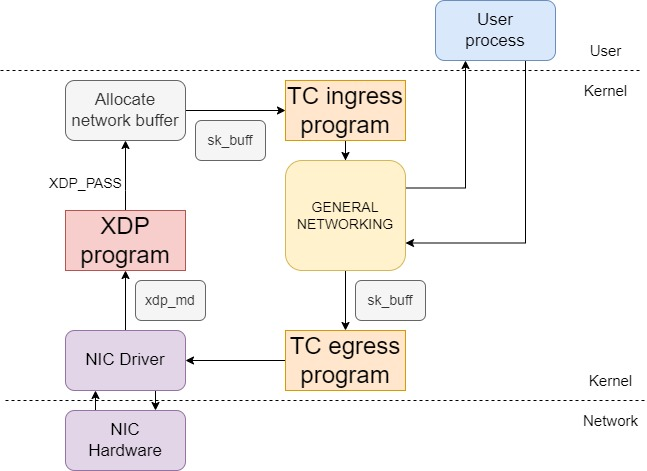
\includegraphics[width=15cm]{xdp_diag.jpg}
	% Either this caption, or change the text afterwards. I still need to know whether to put the long explanation here or on the paragraph, it gets repetitive.
	\caption{Figure showing how the eBPF XDP and TC modules are integrated in the network processing in the Linux kernel.}
	\label{fig:xdp_diag}
\end{figure}

Figure \ref{fig:xdp_diag} shows how XDP is integrated in the network processing of the Linux kernel. After receiving a raw packet (in the figure, \textit{xdp\_md}, which consists on the raw bytes plus some very basic metadata about the packet) from the incoming traffic, XDP program can perform the following actions\cite{xdp_manual}:
\begin{itemize}
\item Analyse the data between the packet buffer bounds.
\item Modify the packet contents, and modify the packet length.
\item Decide between one of the actions displayed in table \ref{table:xdp_actions_av}.
\end{itemize}

\begin{table}[H]
\begin{tabular}{|c|>{\centering\arraybackslash}p{10cm}|}
\hline
ACTION & DESCRIPTION\\
\hline
\hline
XDP\_PASS & Let packet proceed with operated modifications on it.\\
\hline
XDP\_TX & Return the packet at the same NIC it was received from. Packet modifications are kept.\\
\hline
XDP\_DROP & Drops the packet completely, kernel networking will not be notified.\\
\hline
\end{tabular}
\caption{Table showing XDP relevant return values.}
\label{table:xdp_actions_av}
\end{table}

Some of the XDP-exclusive eBPF helpers we will be discussing in later sections are shown in table \ref{table:xdp_helpers}.
\begin{table}[H]
\begin{tabular}{|c|>{\centering\arraybackslash}p{10cm}|}
\hline
eBPF helper & DESCRIPTION\\
\hline
\hline
bpf\_xdp\_adjust\_head() & Enlarges or reduces the extension of a packet, by moving the address of its first byte.\\
\hline
bpf\_xdp\_adjust\_tail() & Enlarges or reduces the extension of a packet, by moving the address of its last byte.\\
\hline
\end{tabular}
\caption{Table showing relevant XDP-exclusive eBPF helpers.}
\label{table:xdp_helpers}
\end{table}


\subsection{Traffic Control}
Traffic Control (TC) programs are also indicated for networking instrumentation. Similarly to XDP, their module is positioned before entering the overall network processing of the kernel. However, as it can be observed in figure \ref{fig:xdp_diag}, they differ in some aspects:
\begin{itemize}
\item TC programs receive a network buffer with metadata (in the figure, \textit{sk\_buff}) about the packet in it. This renders TC programs less ideal than XDP for performing large packet modifications (like new headers), but at the same time the additional metadata fields make it easier to locate and modify specific packet fields\cite{tc_differences}.
\item TC programs can be attached to the \textit{ingress} or \textit{egress} points, meaning that an eBPF program can operate not only over incoming traffic, but also over the outgoing packets.
\end{itemize}

With respect to how TC programs operate, the Traffic Control system in Linux is greatly complex and would require a complete section by itself. In fact, it was already a complete system before the appearance of eBPF. Full documentation can be found at \cite{tc_docs_complete}. For this document, we will explain the overall process needed to load a TC program\cite{tc_direct_action}:
\begin{enumerate}
\item The TC program defines a so-called queuing discipline (qdisc), a packet scheduler that issues packets in a First-In-First-Out (FIFO) order as soon as they are received. This qdisc will be attached to an specific network interface (e.g.: wlan0).
\item Our TC eBPF program is attached to the qdisc. It will work as a filter, being run for every of the packets dispatched by the qdisc.
\end{enumerate}

Similarly to XDP, the TC eBPF programs can decide an action to be executed on a packet by specifying a return value. These actions are almost analogous to the ones in XDP, as it can be observed in table \ref{table:tc_actions}.

\begin{table}[H]
\begin{tabular}{|c|>{\centering\arraybackslash}p{10cm}|}
\hline
ACTION & DESCRIPTION\\
\hline
\hline
TC\_ACT\_OK & Let packet proceed with operated modifications on it.\\
\hline
TC\_ACT\_RECLASSIFY & Return the packet to the back of the qdisc scheduling queue.\\
\hline
TC\_ACT\_SHOT & Drops the packet completely, kernel networking will not be notified.\\
\hline
\end{tabular}
\caption{Table showing TC relevant return values. Full list can be consulted at \cite{tc_ret_list_complete}.}
\label{table:tc_actions}
\end{table}

Finally, as in XDP, there exists a list of useful BPF helpers that will be relevant for the creation of our rootkit. They are shown in table \ref{table:tc_helpers}.
\begin{table}[H]
\begin{tabular}{|c|>{\centering\arraybackslash}p{10cm}|}
\hline
eBPF helper & DESCRIPTION\\
\hline
\hline
bpf\_l3\_csum\_replace() & Recomputes the network layer 3 (e.g.: IP) checksum of the packet.\\
\hline
bpf\_l4\_csum\_replace() & Recomputes the network layer 4 (e.g: TCP) checksum of the packet.\\
\hline
bpf\_skb\_store\_bytes() & Write a data buffer into the packet.\\
\hline
bpf\_skb\_pull\_data() & Reads a sequence of packet bytes into a buffer.\\
\hline
bpf\_skb\_change\_head() & (Only) enlarges the extension of a packet, by moving the address of its first byte.\\
\hline
bpf\_skb\_change\_tail() & Enlarges or reduces the extension of a packet, by moving the address of its last byte.\\
\hline
\hline
\end{tabular}
\caption{Table showing relevant TC-exclusive eBPF helpers.}
\label{table:tc_helpers}
\end{table}


%TODO This section might benefit from some diagrams, maybe. It was a bit to extense already, so skipping it from now
\subsection{Tracepoints} \label{subsection:tracepoints}
Tracepoints are a technology in the Linux kernel that allows to hook functions in the kernel, connecting a 'probe': a function that is executed every time the hooked function is called\cite{tp_kernel}. These tracepoints are set statically during kernel development, meaning that for a function to be hooked, it needs to have been previously marked with a tracepoint statement indicating its traceability. At the same time, this limits the number of tracepoints available.

The list of tracepoint events available depends on the kernel version and can be visited under the directory \textit{/sys/kernel/debug/tracing/events}.

It is particularly relevant for our later research that most of the system calls incorporate a tracepoint, both when they are called (\textit{enter} tracepoint) and when they are exited (\textit{exit} tracepoints). This means that, for a system call sys\_open, both the tracepoint sys\_enter\_open and sys\_exit\_open are available. 

Also, note that the probe functions that are called when hitting a tracepoint receive some parameters related to the context on which the tracepoint is located. In the case of syscalls, these include the parameters with which the syscall was called (only for \textit{enter} syscalls, \textit{exit} ones will only have access to the return value). The exact parameters and their format which a probe function receives can be visited in the file \textit{/sys/kernel/debug/tracing/events/<subsystem>/<tracepoint>/format}. In the previous example with sys\_enter\_open, this is \textit{/sys/kernel/debug/tracing/events/syscalls/sys\_enter\_open/format}.

In eBPF, a program can issue a bpf() syscall with the command BPF\_PROG\_LOAD and the program type BPF\_PROG\_TYPE\_TRACEPOINT, specifying which is the function with the tracepoint to attach to and an arbitrary function probe to call when it is hit. This function probe is defined by the user in the eBPF program submitted to the kernel.

\subsection{Kprobes}
Kprobes are another tracing technology of the Linux kernel whose functionality has been become available to eBPF programs. Similarly to tracepoints, kprobes enable to hook functions in the kernel, with the only difference that it is dynamically attached to any arbitrary function, rather than to a set of predefined positions\cite{kprobe_manual}. It does not require that kernel developers specifically mark a function to be probed, but rather kprobes can be attached to any instruction, with a short list of blacklisted exceptions. 

As it happened with tracepoints, the probe functions have access to the parameters of the original hooked function. Also, the kernel maintains a list of kernel symbols (addresses) which are relevant for tracing and that offer us insight into which functions we can probe. It can be visited under the file \textit{/proc/kallsyms}, which exports symbols of kernel functions and loaded kernel modules\cite{kallsyms_kernel}.

Also similarly, since tracepoints could be found in their \textit{enter} and \textit{exit} variations, kprobes have their counterpart, name kretprobes, which call the hooked probe once a return instruction is reached after the hooked symbol. This means that a kretprobe hooked to a kernel function will call the probe function once it exits.

In eBPF, a program can issue a bpf() syscall with the command BPF\_PROG\_LOAD and the program type BPF\_PROG\_TYPE\_KPROBE, specifying which is the function with the kprobe to attach to and an arbitrary function probe to call when it is hit. This function probe is defined by the user in the eBPF program submitted to the kernel.

\subsection{Uprobes}
Uprobes is the last of the main tracing technologies which has been become accessible to eBPF programs. They are the counterparts of Kprobes, allowing for tracing the execution of an specific instruction in the user space, instead of in the kernel. When the exeuction flow reaches a hooked instruction, a probe function is run. 

For setting an uprobe on an specific instruction of a program, we need to know three components:
\begin{itemize}
\item The name of the program.
\item The address of the function where the instruction is contained.
\item The offset at which the specific instruction is placed from the start of the function.
\end{itemize}

Similarly to kprobes, uprobes have access to the parameters received by the hooked function. Also, the complementary uretprobes also exist, running the probe function once the hooked function returns.

In eBPF, programs can issue a bpf() syscall with the command BPF\_PROG\_LOAD and the program type BPF\_PROG\_TYPE\_UPROBE, specifying the function with the uprobe to attach to and an arbitrary function probe to call when it is hit. This function probe is also defined by the user in the eBPF program submitted to the kernel.

% Is this the best title?
\section{Developing eBPF programs}
In section \ref{section:modern_ebpf}, we discussed the overall architecture of the eBPF system which is now an integral part of the Linux kernel. We also studied the process which a piece of eBPF bytecode follows in order to be accepted in the kernel. However, for an eBPF developer, programming bytecode and working with bpf() calls natively is not an easy task, therefore an additional layer of abstraction was needed. 

Nowadays, there exist multiple popular alternatives for writing and running eBPF programs. We will overview which they are and proceed to analyse in further detail the option that we will use for the development of our rootkit.

\subsection{BCC}
BPF Compiler Collection (BCC) is one of the first and well-known toolkits for eBPF programming available\cite{bcc_github}. It allows to include eBPF code into user programs. These programs are developed in python, and the eBPF code is embedded as a plain string. An example of a BCC program is included in %TODO ANNEX???

Although BCC offers a wide range of tools to easy the development of eBPF programs, we found it not to be the most appropriate for our large-scale eBPF project. This was in particular due to the feature of eBPF programs being stored as a python string, which leads to difficult scalability, poor development experience given that programming errors are detected at runtime (once the python program issues the compilation of the string), and simply better features from competing libraries.

\subsection{Bpftool}
bpftool is not a development framework like BCC, but one of the most relevant tools for eBPF program development. Some of its functionalities include:
\begin{itemize}
\item Loading eBPF programs.
\item List running eBPF programs.
\item Dumping bytecode from live eBPF programs.
\item Extract program statistics and data from programs.
\item List and operate over eBPF maps.
\end{itemize}

Although we will not be covering bpftool during our overview on the constructed eBPF rootkit, it was used extensively during the development and became a key tool for debugging eBPF programs, particularly to peek data at eBPF maps during runtime.

\subsection{Libbpf}
libbpf\cite{libbpf_github} is a library for loading and interacting with eBPF programs, which is currently maintained in the Linux kernel source tree\cite{libbpf_upstream}. It is one of the most popular frameworks to develop eBPF applications, both because it makes eBPF programming similar to common kernel development and because it aims at reducing kernel-version dependencies, thus increasing programs portability between systems\cite{libbpf_core}. During our research, however, we will not make use of this functionalities given that a portable program is not in our research goals.

As we discussed in section \ref{section:modern_ebpf}, eBPF programs are composed of both the eBPF code in the kernel and a user space program that can interact with it. With libbpf, the eBPF kernel program is developed in C (a real program, not a string later compiled as with BCC), while user programs are usually developed in C, Rust or GO. For our project, we will use the C version of libbpf, so both the user and kernel side of our rootkit will be developed in this language.

% Cites in the following paragraph?
When using libbpf with the C language, both the user-side and kernel eBPF program are compiled together using the Clang/LLVM compiler, translating C instructions into eBPF bytecode. As a clarification, Clang is the front-end of the compiler, translating C instructions into an intermediate form understandable by LLVM, whilst LLVM is the back-end compiling the intermediate code into eBPF bytecode. As it can be observed in figure \ref{fig:libbpf}, the result of the compilation is a single program, comprising the user-side which will launch a user process, the eBPF bytecode to be run in the kernel, and other structures libbpf generates about eBPF maps and other meta data. This program is encapsulated as an ELF file (a common executable format).

\begin{figure}[H]
	\centering
	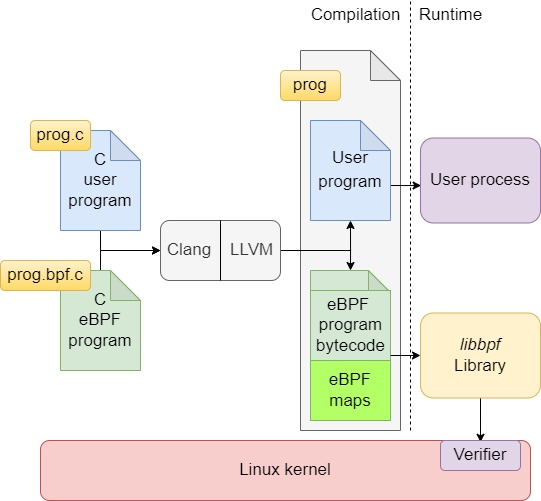
\includegraphics[width=12cm, keepaspectratio=true]{libbpf_prog.jpg}
	\caption{Sketch of the compilation and loading process of a program developed with libbpf.}
	\label{fig:libbpf}
\end{figure}

Finally, we will overview one of the main functionalities of libbpf to simplify eBPF programming, namely the BPF skeleton. This is auto-generated code by libbpf whose aim is to simplify working with eBPF from the user-side program. As a summary, it parses the eBPF programs developed (which may be using different technologies such as XDP, kprobes, TC...) and the eBPF maps used, and as a result offers a simple set of functions for dealing with these programs from the user program. In particular, it allows for loading and unloading an specific eBPF program from user space at runtime.

Table \ref{table:libbpf_skel} describes the API offered by the BPF skeleton. Note that <name> is subtituted by the name of the program being compiled.

\begin{table}[H]
\begin{tabular}{|c|>{\centering\arraybackslash}p{10cm}|}
\hline
Function name & Description\\
\hline
\hline
<name>\_\_open() & Parse the eBPF programs and maps.\\
\hline
<name>\_\_load() & Load the eBPF map in the kernel after its validation, create the maps. However the programs are not active yet.\\
\hline
<name>\_\_attach() & Activate the eBPF programs, attaching them to their corresponding parts in the kernel (e.g. kprobes to kernel functions).\\
\hline
<name>\_\_destroy() & Detach and unload the eBPF programs from the kernel.\\
\hline
\end{tabular}
\caption{Table showing BPF skeleton functions.}
\label{table:libbpf_skel}
\end{table}

Note that the BPF skeleton also offers further granularity at the time of dealing with programs, so that individual programs can be loaded or attached instead of all simultaneously. This is the approach we will generally use in the development of our rootkit, as it will be explained in section \ref{TODO}.







\chapter{Analysis of offensive capabilities}
In the previous chapter, we detailed which functionalities eBPF offers and studied its underlying architecture. As with every technology, a prior deep understanding is fundamental for discussing its security implications. 

Therefore, given the previous background, this chapter is dedicated to an analysis in detail of the security implications of a malicious use of eBPF. For this, we will firstly explore the security features incorporated in the eBPF system. Then, we will identify the fundamental pillars onto which malware can build their functionality. As we mentioned during the project goals, these main topics of research will be the following:
\begin{itemize}
\item Analysing eBPF's possibilities when hooking system calls and kernel functions.
\item Learning eBPF's potential to read/write arbitrary memory.
\item Exploring networking capabilities with eBPF packet filters.
\end{itemize}

Finally, we will study in detail some of the malicious applications that previous researchers have proposed to take advantage of these capabilities of eBPF. In the next chapter, we will proceed to elaborate on these ideas, find new purposes and design our own rootkit.

\section{Security features in eBPF}
As we shown in section \ref{section:modern_ebpf}, eBPF has been an active part of the Linux kernel from its 3.18 version. However, as with many other components of the kernel, its availability to the user depends on the parameters with which the kernel has been compiled. Specifically, eBPF is only available to kernels compiled with the flags specified in table \ref{table:ebpf_kernel_flags}.

\begin{table}[H]
\begin{tabular}{|c|c|>{\centering\arraybackslash}p{8cm}|}
\hline
Flag & Value & Description\\
\hline
\hline
\multicolumn{1}{|c|}{CONFIG\_BPF} & \multicolumn{1}{|c|}{y} & \multirow{2}{*}{Basic BPF compilation (mandatory)}\\
\cline{1-2}
\multicolumn{1}{|c|}{CONFIG\_BPF\_SYSCALL} & \multicolumn{1}{|c|}{m} & \\
\hline
\multicolumn{1}{|c|}{CONFIG\_NET\_ACT\_BPF} & \multicolumn{1}{|c|}{m} & \multirow{2}{*}{Traffic Control functionality}\\
\cline{1-2}
\multicolumn{1}{|c|}{CONFIG\_NET\_CLS\_BPF} & \multicolumn{1}{|c|}{y} & \\
\hline
\multicolumn{1}{|c|}{CONFIG\_BPF\_JIT} & \multicolumn{1}{|c|}{y} & \multirow{2}{*}{Enable JIT compliation}\\
\cline{1-2}
\multicolumn{1}{|c|}{CONFIG\_HAVE\_BPF\_JIT} & \multicolumn{1}{|c|}{y} & \\
\hline
\multicolumn{1}{|c|}{CONFIG\_BPF\_EVENTS} & \multicolumn{1}{|c|}{y} & \multirow{4}{*}{Enable kprobes, uprobes and tracepoints}\\
\cline{1-2}
\multicolumn{1}{|c|}{CONFIG\_KPROBE\_EVENTS} & \multicolumn{1}{|c|}{y} & \\
\cline{1-2}
\multicolumn{1}{|c|}{CONFIG\_UPROBE\_EVENTS} & \multicolumn{1}{|c|}{y} & \\
\cline{1-2}
\multicolumn{1}{|c|}{CONFIG\_TRACING} & \multicolumn{1}{|c|}{y} & \\
\hline
CONFIG\_XDP\_SOCKETS & y & Enable XDP\\
\hline
\end{tabular}
\caption{Kernel compilation flags for eBPF.}
\label{table:ebpf_kernel_flags}
\end{table}

The above table is based on BCC's documentation\ref{table:ebpf_kernel_flags}, but the full list of eBPF-related flags can be extracted in a live system via bpftool, as detailed in Annex \ref{annex:bpftool_flags_kernel}. Nowadays, all mainstream Linux distributions include kernels with full support for eBPF.

\subsection{Access control}

It must be noted that, similarly to kernel modules, loading an eBPF program requires privileged access in the system. In old kernel versions, this means either an user having full root permissions, or having the Linux capability\cite{ubuntu_caps} CAP\_SYS\_ADMIN. Therefore, there existed two main options:
%Should we explain what is a capability?
\begin{itemize}
\item \textbf{Privileged users} can load any kind of eBPF program and use any functionality.
\item \textbf{Unprivileged users} can only load and attach eBPF programs of type BPF\_PROG\_TYPE\_SOCKET\_FILTER\cite{evil_ebpf_p9}, offering the very limited functionality of filtering packets received on a socket.
\end{itemize}

More recently, in an effort to further granulate the permissions needed for loading, attaching and running eBPF programs, CAP\_SYS\_ADMIN has been substituted by more specific capabilities\cite{ebpf_caps_intro}\cite{ebpf_caps_lwn}. The current system is therefore described in table \ref{table:ebpf_caps_current}.

\begin{table}[H]
\begin{tabular}{|>{\centering\arraybackslash}p{4cm}|>{\centering\arraybackslash}p{10cm}|}
\hline
Capabilities & eBPF functionality\\
\hline
\hline
No capabilities & Load and attach BPF\_PROG\_TYPE\_SOCKET\_FILTER, load BPF\_PROG\_TYPE\_CGROUP\_SKB programs.\\
\hline
CAP\_BPF & Load (but not attach) any type of program, create most types of eBPF map and access them if their id is known\\
\hline
CAP\_NET\_ADMIN & Attach networking programs (Traffic Control, XDP, ...)\\
\hline
CAP\_PERFMON & Attaching kprobes, uprobes and tracepoints. Read access to kernel memory.\\
\hline
CAP\_SYS\_ADMIN & Privileged eBPF. Includes iterating over eBPF maps, and CAP\_BPF, CAP\_NET\_ADMIN, CAP\_PERFMON functionalities.\\
\hline
\end{tabular}
\caption{Capabilities needed for eBPF.}
\label{table:ebpf_caps_current}
\end{table}

Therefore, eBPF network programs usually require both CAP\_BPF and CAP\_NET\_ADMIN, whilst tracing programs require CAP\_BPF and CAP\_PERFMON. CAP\_SYS\_ADMIN still remains as the (non-preferred) capability to assign to eBPF programs with complete access in the system.

Although for a long time there have existed efforts towards enhancing unprivileged eBPF, it remains a worrying feature\cite{unprivileged_ebpf}. The main issue is that the verifier must be prepared to detect any attempt to extract kernel memory access or user memory modification by unprivileged eBPF programs, which is a complex task. In fact, there have existed numerous security vulnerabilities which allow for privilege escalation using eBPF, that is, execution of privileged eBPF programs by exploiting vulnerabilities in unprivileged eBPF\cite{cve_unpriv_ebpf}.

This influx of security vulnerabilities leads to the recent inclusion of an attribute into the kernel which allows for setting whether unprivileged eBPF is allowed in the system or not. This parameter is named \textit{kernel.unprivileged\_bpf\_disabled}, its values can be seen in table \ref{table:unpriv_ebpf_values}.

\begin{table}[H]
\begin{tabular}{|>{\centering\arraybackslash}p{4cm}|>{\centering\arraybackslash}p{10cm}|}
\hline
Value & Meaning\\
\hline
\hline
0 & Unprivileged eBPF is enabled.\\
\hline
1 & Unprivileged eBPF is disabled. A system reboot is needed to enable it after changing this value.\\
\hline
2 & Unprivileged eBPF is disabled. A system reboot is not needed to enable it after changing this value.\\
\hline
\end{tabular}
\caption{Values for unprivileged eBPF kernel parameter.}
\label{table:unpriv_ebpf_values}
\end{table}

Nowadays, most Linux distributions have set value 1 to this parameter, therefore disallowing unprivileged eBPF completely. These include Ubuntu\cite{unpriv_ebpf_ubuntu}, Suse Linux\cite{unpriv_ebpf_suse} or Red Hat Linux\cite{unpriv_ebpf_redhat}, between others.

\subsection{eBPF maps security}
In table \ref{table:ebpf_caps_current}, we observed that only programs with CAP\_SYS\_ADMIN are allowed to iterate over eBPF maps. The reason why this is restricted to privileged programs is because it is functionality that is a potential security vulnerability, which we will now proceed to analyse.

In subsection \ref{subsection:ebpf_maps} we mentioned that eBPF maps are opened by specifying an ID (which works similarly to the typical file descriptors), while in table \ref{table:ebpf_map_types} we showed that, for performing operations over eBPF maps using the bpf() syscall, the map ID must be specified too. 

Map IDs are known by a program after creating the eBPF map, however, a program can also explore all the available maps in the system by using the BPF\_MAP\_GET\_NEXT\_ID operation in the bpf() syscall, which allows for iterating through a complete hidden list of all the maps created. This means that privileged programs can find and have read and write access to any eBPF map used by any program in the system.

Therefore, a malicious privileged eBPF program can access and modify other programs' maps, which can lead to:
\begin{itemize}
\item Modify data used for the program operation. This is the case for maps which mainly store data structures, such as BPF\_MAP\_TYPE\_HASH.
\item Modify the program control flow, altering the instructions executed by an eBPF program. This can be achieved if a program is using the bpf\_tail\_call() helper (introduced in table \ref{table:ebpf_helpers}) which is taking data from a map storing eBPF programs (BPF\_MAP\_TYPE\_PROG\_ARRAY, introduced in table \ref{table:ebpf_map_types}).
\end{itemize}


\section{Abusing tracing programs}
eBPF tracing programs (kprobes, uprobes and tracepoints) are hooked to specific points in the kernel or in the user space, and call probe functions once the flow of execution reaches the instruction to which they are attached. This section details the main security concerns regarding this type of programs.

\subsection{Access to function arguments}
As we saw in section \ref{section:ebpf_prog_types}, tracing programs receive as a parameter those arguments with which the hooked function originally was called. These parameters are read-only and thus, in principle, they cannot be modified inside the tracing program (we will show this is not entirely true in section \ref{section:mem_corruption}). The next code snippets show the format in which parameters are received when using libbpf (Note that libbpf also includes  some macros that offer an alternative format, but the parameters are the same).


\begin{lstlisting}[language=C, caption={Probe function for a kprobe on the kernel function vfs\_write.}, label={code:format_kprobe}]
SEC("kprobe/vfs_write")
int kprobe_vfs_write(struct pt_regs* ctx){
\end{lstlisting}

\begin{lstlisting}[language=C, caption={Probe function for an uprobe, execute\_command is defined from user space.}, label={code:format_uprobe}]
SEC("uprobe/execute_command")
int uprobe_execute_command(struct pt_regs *ctx){
\end{lstlisting}

\begin{lstlisting}[language=C, caption={Probe function for a tracepoint on the start of the syscall sys\_read.}, label={code:format_tracepoint}]
SEC("tp/syscalls/sys_enter_read") 
int tp_sys_enter_read(struct sys_read_enter_ctx *ctx) { 
\end{lstlisting}

In code snippets \ref{code:format_kprobe} and \ref{code:format_uprobe} we can identify that the parameters are passed to kprobe and uprobe programs as a pointer to a \textit{struct pt\_regs*}. This struct contains as many attributes as registers exist in the system architecture, in our case x86\_64. Therefore, on each probe function, we will receive the state of the registers at the original hooked function. This explains the format of the \textit{struct pt\_regs}, shown in code snippet \ref{code:format_ptregs}:

\begin{lstlisting}[language=C, caption={Format of struct pt\_regs.}, label={code:format_ptregs}]
struct pt_regs {
	long unsigned int r15;
	long unsigned int r14;
	long unsigned int r13;
	long unsigned int r12;
	long unsigned int bp;
	long unsigned int bx;
	long unsigned int r11;
	long unsigned int r10;
	long unsigned int r9;
	long unsigned int r8;
	long unsigned int ax;
	long unsigned int cx;
	long unsigned int dx;
	long unsigned int si;
	long unsigned int di;
	long unsigned int orig_ax;
	long unsigned int ip;
	long unsigned int cs;
	long unsigned int flags;
	long unsigned int sp;
	long unsigned int ss;
};
\end{lstlisting}

By observing the value of the registers, we are able to extract the parameters of the original hooked function. This can be done by using the System V AMD64 ABI\cite{8664_params_abi}, the calling convention used in Linux. Depending on whether we are in the kernel or in user space, the registers used to store the values of the function arguments are different. Table \ref{table:systemv_abi} summarizes these two interfaces. Some other relevant registers are also displayed as a reference in table \ref{table:systemv_abi_other}.

\begin{table}[H]
\begin{tabular}{|>{\centering\arraybackslash}p{2cm}|>{\centering\arraybackslash}p{3cm}|}
\hline
\multicolumn{2}{|c|}{User interface}\\
\hline
Register & Purpose\\
\hline
\hline
rdi & 1st argument\\
\hline
rsi & 2nd argument\\
\hline
rdx & 3rd argument\\
\hline
rcx & 4th argument\\
\hline
r8 & 5th argument\\
\hline
r9 & 6th argument\\
\hline
rax & Return value\\
\hline
\end{tabular}
\quad
\begin{tabular}{|>{\centering\arraybackslash}p{2cm}|>{\centering\arraybackslash}p{3cm}|}
\hline
\multicolumn{2}{|c|}{Kernel interface}\\
\hline
Register & Purpose\\
\hline
\hline
rdi & 1st argument\\
\hline
rsi & 2nd argument\\
\hline
rdx & 3rd argument\\
\hline
r10 & 4th argument\\
\hline
r8 & 5th argument\\
\hline
r9 & 6th argument\\
\hline
rax & Return value\\
\hline
\end{tabular}
\caption{Argument passing convention of registers for function calls in user and kernel space respectively.}
\label{table:systemv_abi}
\end{table}


\begin{table}[H]
\begin{tabular}{|>{\centering\arraybackslash}p{2cm}|>{\centering\arraybackslash}p{10cm}|}
\hline
Register & Purpose\\
\hline
\hline
rip & Instruction Pointer - Memory address of the next instruction to execute\\
\hline
rsp & Stack Pointer - Memory address where next stack operation takes place\\
\hline
rbp & Base/Frame Pointer - Memory address of the start of the stack frame\\
\hline
\end{tabular}
\caption{Other relevant registers in x86\_64 and their purpose.}
\label{table:systemv_abi_other}
\end{table}

In the case of tracepoints, we can see in code snippet \ref{code:format_tracepoint} that it receives a \textit{struct sys\_read\_enter\_ctx*}. This struct must be manually defined, as explained in \ref{subsection:tracepoints}, by looking at the file \textit{/sys/kernel/debug/tracing/events/syscalls/sys\_enter\_read/format}. Code snippet \ref{code:sys_enter_read_tp} shows the format of the struct.

\begin{lstlisting}[language=C, caption={Format for parameters in sys\_enter\_read specified at the format file.}, label={code:sys_enter_read_tp_format}]
field:unsigned short common_type; offset:0; size:2; signed:0;
field:unsigned char common_flags; offset:2; size:1; signed:0;
field:unsigned char common_preempt_count; offset:3; size:1; signed:0;
field:int common_pid; offset:4; size:4; signed:1;
field:int __syscall_nr;	offset:8; size:4; signed:1;
field:unsigned int fd; offset:16; size:8; signed:0;
field:char * buf; offset:24; size:8; signed:0;
field:size_t count; offset:32; size:8; signed:0;
\end{lstlisting}

\begin{lstlisting}[language=C, caption={Format of custom struct sys\_read\_enter\_ctx.}, label={code:sys_enter_read_tp}]
struct sys_read_enter_ctx {
    unsigned long long pt_regs;
    int __syscall_nr;
    unsigned int padding;
    unsigned long fd;
    char* buf;
    size_t count;
};
\end{lstlisting}

As we can observe, we are given a set of attributes which include the parameters with which the syscall was called. Moreover, we can still obtain an address pointing to another \textit{struct pt\_regs}, as in kprobes and uprobes, by combining the first four fields and considering it as a 32-bit long address. This means we will still be able to extract the value of the rest of the registers too. 

It must be noted that, in syscalls, in addition to use the kernel parameter passing convention specified in table \ref{table:systemv_abi}, the number specifying the syscall must be passed in register rax too.

On a final note, as we mentioned in section \ref{section:ebpf_prog_types}, there exist differences in the parameters received in probe functions depending on the two variations of tracing programs. Therefore:
\begin{itemize}
\item kprobe, uprobe and \textit{enter} tracepoints will receive the full parameters as we specified before, but not the return value of the function (since it is not executed yet).
\item kretprobes, uretprobes and \textit{exit} tracepoints will still receive the \textit{struct pt\_regs}, but without any of the parameters and with only the return value of the function.
\end{itemize}

Taking into account all the previous, the fact that tracing programs have read-only access to function arguments can be considered an useful and needed feature for tracing applications, but malicious eBPF can use this for purposes such as:
\begin{itemize}
\item Gather kernel and user data passed to a function as a parameter. In many cases this information can be potentially interesting for an attacker, such as passwords.
\item Store in eBPF maps information about system activities, to be used by other malicious eBPF programs.
\end{itemize}

Usually, since many function arguments are pointers to user or kernel addresses (such as buffers where a string or a struct with data is located), eBPF tracing programs can use two eBPF helpers that enable to read large byte arrays from both kernel and user space:
\begin{itemize}
\item bpf\_probe\_read\_user()
\item bpf\_probe\_read\_kernel()
\end{itemize}

These helpers, previously introduced in table \ref{table:ebpf_helpers}, enable to read an arbitrary number of bytes from an user or kernel address respectively, allowing us to extract the information pointed by the parameters received by eBPF programs.

\subsection{Reading memory out of bounds}
As we introduced in the previous subsection, the bpf\_probe\_read\_user() and bpf\_probe\_read\_kernel() helpers can be used to access memory of pointers received as parameters in the hooked functions. 

However, although in general the eBPF verifier attempts to reject illegal memory accesses, it does not prevent a malicious program from passing an arbitrary memory address (in kernel or user space) to the above helpers. This means that an eBPF program can potentially read any address in user or kernel space, (as long as it is marked as readable in the corresponding memory pages). Furthermore, an attacker can locate specific data structures and memory sections by taking the function parameter as a reference point in memory.

A particularly relevant case (which we will later use for our rootkit) involves accessing user memory via the parameters of tracepoints attached at system calls. Provided the nature of syscalls, whose purpose is to communicate user and kernel space, all parameters received will belong to the user space, and therefore any pointer passed will be an address in user memory. This enables an eBPF program to get a foothold into the virtual address space of the process calling the syscall, which it can proceed to scan looking for data or specific instructions. This technique will be further elaborated in section \ref{TODO}.

\subsection{Overriding function return values}
A potentially dangerous functionality in eBPF tracing programs is the ability to modify the return value of kernel functions\cite{ebpf_friends_p15}\cite{ebpf_override_return}. This can be done via the eBPF helper bpf\_override\_return, and it works exclusively from kretprobes.

Apart from only working on kretprobes, additional restrictions are applied to this helper. It will only work if the kernel was compiled with the CONFIG\_BPF\_KPROBE\_OVERRIDE flag, and only if the kretprobe is attached to a function to which, during the kernel development, the macro ALLOW\_ERROR\_INJECTION() has been indicated. Currently, only a small selection of functions include this macro, but most system calls can be found to implement it. The following code snippets show how a system call like sys\_open is defined in kernel v5.11:

\begin{lstlisting}[language=C, caption={Definition of the syscall sys\_open in the kernel \cite{code_kernel_open}}, label={code:override_return_1}]
SYSCALL_DEFINE3(open, const char __user *, filename, int, flags, umode_t, mode)
{
	if (force_o_largefile())
		flags |= O_LARGEFILE;
	return do_sys_open(AT_FDCWD, filename, flags, mode);
}
\end{lstlisting}

\begin{lstlisting}[language=C, caption={Definition of the macro for creating syscalls, containing the error injection macro. Only relevant instructions included, complete macro can be found in the kernel \cite{code_kernel_open}}, label={code:override_return_2}]
#define SYSCALL_DEFINE3(name, ...) SYSCALL_DEFINEx(3, _##name, __VA_ARGS__)
#ifndef __SYSCALL_DEFINEx
#define __SYSCALL_DEFINEx(x, name, ...)\
	[...]
	ALLOW_ERROR_INJECTION(sys##name, ERRNO);\
	[...]
\end{lstlisting}


By looking at snippets \ref{code:override_return_1} and \ref{code:override_return_2}, we can observe that the system call sys\_open involves the inclusion of the ALLOW\_ERROR\_INJECTION macro. Therefore, any kretprobe attached to a system call function will be able to modify its return value.

In order to be able to modify the return value of functions, the aforementioned eBPF helper makes use of the fault injection framework of the Linux kernel\cite{fault_injection}, which was created before eBPF itself, and whose original purpose is to allow for generating errors in kernel programs for debugging purposes.

Taking the previous information into account, we can find that a malicious eBPF program, by tampering with the kernel-user space interface which are system calls, can mislead user programs, which trust the output of kernel code. This can lead to:
\begin{itemize}
\item A program believes a system call exited with an error, while in reality the kernel completed the operation with success, or viceversa. For instance, the result of a call to sys\_open can mislead a user program into thinking that a file does not exist.
\item A program receives incorrect data on purpose. For instance, a buffer may look empty or of a reduced size upon a sys\_read call, while in reality more data is available to be read.
\end{itemize}

\subsection{Sending signals to user programs}
Another eBPF helper that is subject to malicious purposes is bpf\_send\_signal. This helper enables to send an arbitrary signal to the thread of the process running a hooked function.

Therefore, this helper can be used to forcefully terminate running user processes, by sending the SIGKILL signal. In this way, combined with the observability into the parameters received at a call, a malicious eBPF can kill and deactivate processes to favour its malicious purposes.

\subsection{Conclusion}
As a summary, a malicious eBPF program loaded and attached as a tracing program undermines the existing trust between user programs and the kernel space. 

Its ability to access sensitive data in function parameters and reading arbitrary memory can lead to gathering extensive information on the running processes of a system, whilst the malicious use of eBPF helpers means the modification of the data passed to the user space, and the control over which programs are allowed to be running on the system.

\section{Memory corruption} \label{section:mem_corruption}
Privileged malicious eBPF programs (or those with the CAP\_BPF + CAP\_PERFMON capabilities) have the potential to get:
\begin{itemize}
\item Read and write access in user memory.
\item Read-only access in kernel memory.
\end{itemize}


\subsection{Accessing user memory}


%TODO Talk about the difference between having always on BPF and always on kernel modules (maybe this is better in the introduction)


\chapter{Methods??}
%M-> Following the particular TFG we discussed and also others, it looks like the main chapter(s) varies name depending on the TFG topic. Also is there a prefered way to distribute this?


\chapter{Results}


\chapter{Conclusion and future work}




%----------
%	BIBLIOGRAPHY
%----------	

%\nocite{*} % Si quieres que aparezcan en la bibliografía todos los documentos que la componen (también los que no estén citados en el texto) descomenta está lína

\clearpage
\addcontentsline{toc}{chapter}{Bibliography}

\printbibliography



%----------
%	ANEX
%----------	

%M-> Mentioned putting some demos and PoCs here...
%

%Including bpftool commands here to be referenced. Is it a good idea?


\chapter* {Appendix A - Bpftool commands} \label{annex:bpftool_flags_kernel}
\pagenumbering{gobble} % Las páginas de los anexos no se numeran
\section*{eBPF-related kernel compilation flags} 
\begin{lstlisting}[language=bash]
$ bpftool feature
\end{lstlisting}

\begin{verbatim}
CONFIG_BPF is set to y
CONFIG_BPF_SYSCALL is set to y
CONFIG_HAVE_EBPF_JIT is set to y
CONFIG_BPF_JIT is set to y
CONFIG_BPF_JIT_ALWAYS_ON is set to y
CONFIG_CGROUPS is set to y
CONFIG_CGROUP_BPF is set to y
CONFIG_CGROUP_NET_CLASSID is set to y
CONFIG_SOCK_CGROUP_DATA is set to y
CONFIG_BPF_EVENTS is set to y
CONFIG_KPROBE_EVENTS is set to y
CONFIG_UPROBE_EVENTS is set to y
CONFIG_TRACING is set to y
CONFIG_FTRACE_SYSCALLS is set to y
CONFIG_FUNCTION_ERROR_INJECTION is set to y
CONFIG_BPF_KPROBE_OVERRIDE is set to y
CONFIG_NET is set to y
CONFIG_XDP_SOCKETS is set to y
CONFIG_LWTUNNEL_BPF is set to y
CONFIG_NET_ACT_BPF is set to m
CONFIG_NET_CLS_BPF is set to m
CONFIG_NET_CLS_ACT is set to y
CONFIG_NET_SCH_INGRESS is set to m
CONFIG_XFRM is set to y
CONFIG_IP_ROUTE_CLASSID is set to y
CONFIG_IPV6_SEG6_BPF is set to y
CONFIG_BPF_LIRC_MODE2 is not set
CONFIG_BPF_STREAM_PARSER is set to y
CONFIG_NETFILTER_XT_MATCH_BPF is set to m
CONFIG_BPFILTER is set to y
CONFIG_BPFILTER_UMH is set to m
CONFIG_TEST_BPF is set to m
CONFIG_HZ is set to 250
\end{verbatim}


\chapter* {Appendix B}


\end{document}
